\documentclass{standalone}
\usepackage{tikz}
\usetikzlibrary{calc, intersections}

\begin{document}
	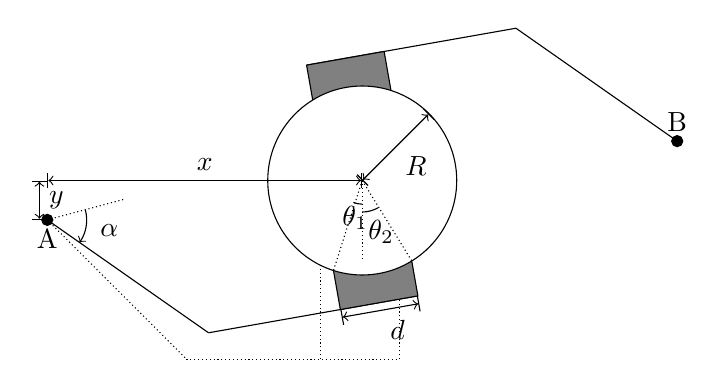
\begin{tikzpicture}[auto]
	
	\draw[fill] (-4, -.5) node[below] {A} circle (2pt);
	%\draw[|<->|] (-.5, -2.1) -- node[swap] {$l$} (.5, -2.1);
	\draw (-4,-.5) -- +(-35:2.5) coordinate (f);
	
	\draw[densely dotted] (-4,-.5) -- +(-45:2.5) coordinate (f');
	\draw[densely dotted] (f') -- +(1.7,0) coordinate (a') -- +(2.7,0) coordinate (b');
	\draw[densely dotted] (a') -- +(0,1.5) (b') -- +(0,1);	
	\draw (f) -- +(10:1.7) coordinate (a) -- +(10:2.7) coordinate (b);
	\draw[|<->|] ($ (a)+(280:.1) $) -- node[swap] {$d$} ($ (b)+(280:.1) $);
	\draw[name path=l1, fill=gray] (b) -- ++(100:1) -- ++ (190:1) -- (a) -- cycle;
	\draw[fill] (4,.5) node[above] {B} circle (2pt);
	\draw (4,.5) --+(145:2.5) coordinate (g);
	\draw (g) -- + (190:1.7) coordinate (c) --+ (190:2.7) coordinate (d);
	\draw[name path=l2, fill=gray] (c) -- ++(280:1) -- ++(190:1) -- (d) -- cycle;
	
	\draw[fill=white, name path=circle] (0,0) circle (1.2);
	
	\draw[|<->|] (0,0) -- node[swap] {$R$} (45:1.2);
	%\draw[|<->|] (1.35, 0) --node {$h$} (1.35,0 |-a');
	
	\path[name intersections={of=l1 and circle, by={x1, x2}}];
	\draw[densely dotted, name path=radi1] (0,0) -- (x1);
	\draw[densely dotted, name path=radi2] (0,0) -- (x2);
	\draw[densely dotted] (0,0) -- (0, -1);
	\path[name path=arc1] (0, -0.2) arc (-180:-90:0.2);
	\path[name path=arc2] (0, -0.2) arc (-90:0:0.2);
	\path[name intersections={of=radi1 and arc1, by=a1}];
	\path[name intersections={of=radi2 and arc2, by=a2}];
	\draw (0, -0.4) arc (-90:-60:0.4);
	\draw (0, -0.3) arc (-90:-112:0.3);
	\node at (-70:0.7) {$\theta_2$};
	\node at (-101:0.48) {$\theta_1$};
	
	\draw[|<->|] (0,0) --node[swap] {$x$} (-4,0);
	\draw[|<->|] (-4.1,0) -- node {$y$} (-4.1, -.5);
	
	%\node at (0,0) {commutator};
	\draw[densely dotted] (-4,-.5) -- +(15:1);
	\draw[->] (-4, -.5) +(15:.5) arc (15:-35:.5);
	\node at ($ (-4,-.5) +(-10:.8) $) {$\alpha$};

	\end{tikzpicture}
		
\end{document}